%%% Fiktivní kapitola s ukázkami sazby

\chapter{Implementace}

Kapitola implementace se věnuje konkrétním akcím vedoucím k vytvoření spustitelného aplikačního artefaktu. V jednotlivých podkapitolách budou uvedeny využité prostředky, konkrétní kroky a jejich výstupy. Některé z těchto kroků jsou použitelné pro všechny Expo projekty a některé úsudky lze využít při vytváření vlastních Expo projektů. Za zmínku zde také stojí kapitola Implementace off-line map, ve které je popsán způsob jak zajistit funkční off-line mapy pro Expo projekty, pro co neexistují zatím žádné komunitní knihovny nebo Expo-nativní způsoby řešení.

\section{Vývojové prostředí}

% https://www.techopedia.com/definition/16376/development-environment

Vývojové prostředí je kolekce procedur a nástroj pro vývoj, testování a ladění aplikací nebo programů \cite{technopediaDevEnv}. Termín vývojové prostředí se používá v synonymu s termínem IDE, integrovaným vývojový prostředím, což je softwarový nástroj pro psaní, sestavení, testování a ladění programů. Do tohoto termínu taktéž lze zahrnout i nástroje co IDE samotné využívá pro setavení artefaktů.

Pro vývoj aplikace byly zvoleny následující nástroje vývojového prostředí:

\begin{itemize}
	\item VisualStudio Code jako nástroj IDE,
	\item Git jako verzovací nástroj,
	\item GitHub jako nástroj verzování i projektového řízení,
	\item AndroidStudio pro správu Android virtuálních strojů,
	\item XCode pro správu iOS virtuálních strojů (pouze na MacOS).
\end{itemize}

Dalším klíčovým softwarovým nástrojem je taktéž instalace Node.js a balíčkovacího nástroje NPM, bez kterých by byl vývoj Expo aplikace nemožný. Text této práce se jejich instalaci nevěnuje a předpokládá, že již nainstalované jsou. Instalace na běžných a aktuálních verzích OS není problémem.

Do pojmu vývojové prostředí se zahrnují i izolovaná prostředí, ve kterém běží testovací nebo produkční instance aplikace (resp. datového zdroje), v tomto případě platformy Anitra. Pro vývoj této aplikace nebylo toto rozlišení nutné a vyvíjelo se přímo na produkční verzi platformy Anitra.

\subsection{Vytvoření projektu}

V ukázce kódu \ref{expoinstall} bylo již zmíněno, jakým způsobem vytvořit Expo projekt. Pro vytvoření expo projektu stačí zadat následující příkazy do příkazové řádky.

\begin{lstlisting}[language=Bash, caption=Vytvoření nového projektu]
npm install --global expo-cli
expo init mobilni-aplikace
\end{lstlisting}

První řádek nainstaluje \emph{expo-cli}, nástroje pro vytváření, správu, spouštění a sestavení Expo projektů. Druhý příkaz vytvoří nový expo projekt \emph{mobilni-aplikace} v aktuální složce uživatele.

Z předpřipraveného kódu je dobré zmínit vstupní bod aplikace \emph{App.tsx}, ve kterém je připravená ukázková komponenta. Z tohoto vstupního bodu se implementují navigátory zmíněné v kapitole Implementace navigátorů.

\section{Implementace úložišť a entit}

Implementace úložišť a entit byla vytvořena dle návrhu aplikace. Bylo vytvořeno více entit, než bylo plánováno, aby celá aplikace komunikovala za pomocí typovaných objektů a tím se zjednodušil proces ladění v aplikaci i urychlil vývoj. Pro entity bylo využito rozhraní, aby entity pro funkce ukládání měly stejnou signaturu a bylo je možné používat ve stylu OOP bez složitých konstrukcí. V ukázce kódu uvedené níže je ukázáno rozhraní, které musí implementovat všechny entity a entity, které mají být uložitelné na disk.

\begin{lstlisting}[language=JavaScript, caption=Ukázka entity]
export interface IEntity {
	id?: number;
	
	synchronized: boolean;
	lastSynchronized?: Date;
};

export interface ISerializableEntity extends IEntity {
	toJson() : object;
	
	toJsonString() : string;
	
	fromJson(json: any): IEntity;
};
\end{lstlisting}

Implementace úložišť samotných spočívá v implementaci tří částí -- v komunikaci se serverem, transformaci dat od serveru a uložení těchto dat na disk. Pro komunikaci se serverem pomocí HTTP Rest API byla zvolena knihovna \emph{axios}, která se běžně používá v JavaScriptových projektech pro abstrakci rozdílů mezi jednotlivými klienty. Knihovna dále umožňuje jednodušší přístup např. k hlavičkám HTTP dotazu a je tedy jednoduché se např. oproti vzdálenému serveru autentifikovat. Axios očekává na vstupu objekt obsahující výčet parametrů a na výstupu vrací tělo dotazu zformátované do správného formátu (např. když server vrací JSON odpověď, Axios z vráceného textu správně složí JSON).

Transformace dat ze serveru spočívá v převodu klíčů a hodnot vrácených ze serveru do předem zmíněných entit. Entity v aplikaci neobsahují celá data, ale pouze výčet, který aplikace skutečně potřebuje. Tímto se šetří nejen místo na disku, ale i doba serializace a deserializace entit při čtení z disku. V API nejde stanovit, jaká pole dotazovatel vyžaduje a filtrování je tedy nutno provést až na koncovém bodu procesu, tedy v mobilní aplikaci.

Pro uložení dat byla využita součást Expo \emph{expo-file-system}, která abstrahuje od jednotlivých souborových systémů operačních systémů. Nevýhodou tohoto systému je neobratnost při zakládání složek, složky se musí vytvářet dopředu a nelze je vytvořit při zápisu souboru. Podstatnější nevýhodou je nutnost serializovat obsah souboru do textu, a nejedná se tedy o příliš vhodnou metodu ukládání např. obrazových dat kvůli nutnosti převést binární data na textový formát např. Base64. Alternativní řešení pro Expo neexistuje. Ukázka práce se souborovým systémem je v následující ukázce kódu.

\begin{lstlisting}[language=JavaScript, caption=Ukázka entity]
import * as FileSystem from 'expo-file-system';

let string = await FileSystem.readAsStringAsync(path);
\end{lstlisting}

Do proměnné string se asynchronně zapíše obsah souboru v cestě, v případě chyby čtení, např. způsobené neexistujícím souborem, se vyhodí výjimka. Soubor lze dále zpracovat předevím např. textu na JSON nebo na XML, případně jakýkoliv jiný formát, který aplikace využívá. V aplikaci se nad těmito funkcemi staví třída PersistenStorage, která poskytuje obecné metody pro uložení a získání kolekcí či jednotlivých entit.

\section{Implementace obrazovek}

Implementace obrazovek byla nejdelší částí tvorby aplikace a nejnáročnější na testování. Obrazovky jsou React komponenty umístěny ihned pod navigátorem. V jejich životním cyklu se vytváří subkomponenty, získávají data z úložišť a pomocí událostí komunikují s úložišti. Obrazovky jsou spolu se subkomponentami zodpovědné za správu interakcí s uživatelem.

Níže je uvedena ukázková implementace obrazovky AuthLoading, která rozhoduje o přesměrování uživatele po zapnutí aplikace, pokud je přihlášen či ne.

\begin{lstlisting}[language=JavaScript, caption=Ukázka implementace obrazovky]
import React from 'react';
import { StyleSheet, Text, View } from 'react-native';
import { MaterialIndicator } from 'react-native-indicators';

import AuthStore from '../store/AuthStore';
import Theme from "../constants/Theme.js";

export default class AuthLoading extends React.Component {
	verifyAuth = async () => {
		await AuthStore.awaitAuth();
		if (AuthStore.isAuthorized) {
			this.props.navigation.navigate("Map");
		} else {
			this.props.navigation.navigate("AuthContainer");
		}
	}
	
	componentDidMount() {
		this.verifyAuth();
	}
	
	render () {
		return (
		<View style={styles.container}>
			<View>
				<MaterialIndicator color={ Theme.colors.brand.primary }/>
			</View>
		</View>
		);
	}
}

const styles = StyleSheet.create({
	container: {
		flex: 1,
		backgroundColor: Theme.colors.default.background,
		alignItems: 'center',
		justifyContent: 'center',
		alignSelf: 'stretch',
	}
});

\end{lstlisting}

V ukázce lze vidět několik podstatných částí. V první části jsou importy závislostí, kde veškeré obrazovky potřebují naimportovat alespoň závislost \emph{React} z knihovny React. Na druhém řádku lze vidět import typických ovládacích prvků a utilit pro obrazovku či subkomponentu. StyleSheet je způsob zapsání stylu pro ReactNative, ukázka způsobu zápisu stylů se nachází v objektu \emph{styles} na konci ukázky kódu. Text je komponenta, která umožňuje zobrazení stylovaného textu a jako jediná může obsahovat čistý text. Komponenta View rámcově odpovídá funkci tagu \emph{div} v HTML a je pouze prázdným kontejnerem pro ostatní komponenty, ale může být stylována. Následně je vidět import \emph{MaterialIndicator} z knihovny \emph{react-native-indicators}, externí komponenty, která zobrazuje načítací spinner, aby UI nevypadala neresponzivně. Následně je importováno úložiště pro autentifikaci a seznam konstant obsahující styl aplikace.

Samotná obrazovka začíná na řádku 8, kde se nachází definice třídy komponenty. Na řádku devět se nachází metoda komponenty, ve které se volá úložiště Auth pro ověření, zda je uživatel autorizovaný, a případně se přenaviguje na správnou obrazovku. Vysoce podstatná je metoda \emph{componentDidMount} na řádku 18, která se spustí po načtení komponenty a volá již zmiňovanou funkci na ověření přihlášení. Metoda render vrací JSX obrazovky, tedy strukturu všech subkomponent. Na konci je již zmiňovaný objekt styles, obsahující styly.

Tato obrazovka je reprezentativní pro všechny obrazovky, s výjimkou hlavní mapy.

\subsection{Implementace hlavní mapy}

Pro hlavní část této obrazovky, tedy mapy, byla využita knihovna \emph{react-native-maps} z důvodu absence alternativ pro Expo. Knihovna však splňuje veškeré požadavky aplikace. Do mapy lze např. vkládat objekty typu trasa, bod i tyto body následně stylovat. Objekty do mapy se přidávají jako individuální komponenty, např. bod s tzv. infoboxem (bublinou nad bodem) se vytvoří následujícím způsobem.

\begin{lstlisting}[language=JavaScript, caption=Ukázka implementace obrazovky]
<MapView>
	<Marker
		coordinate={ { latitude: point.lat, longitude: point.lng } }
		icon={image}
		image={image}
		zIndex={zIndex}
	>
		<Callout>
			<MarkerPosition tracking={track.tracking} id={point.id}/>
		</Callout>
	</Marker>
</MapView>
\end{lstlisting}

Ukázka ilustruje způsob umístění v mapě (parametr coordinate), způsob vybrání ikony pro obě platformy (parametr icon a image) a nastavení zIndexu, který určuje pořadí vykreslování komponent vzájemně se překrývajících. Komponenta Callout obsahuje již zmiňované infowindow, které obsahuje subkomponentu MarkerPosition.

Pro implementaci vyjížděcího menu pro filtry byla využita komponenta \emph{rn-sliding-up-panel}, která plně splina zadání z kapitoly návrh. Detaily implementace lze zobrazit v příloze, jelikož jsou příliš dlouhé pro ukázky v textu této práce.

\begin{figure}[H]
	\begin{center}
		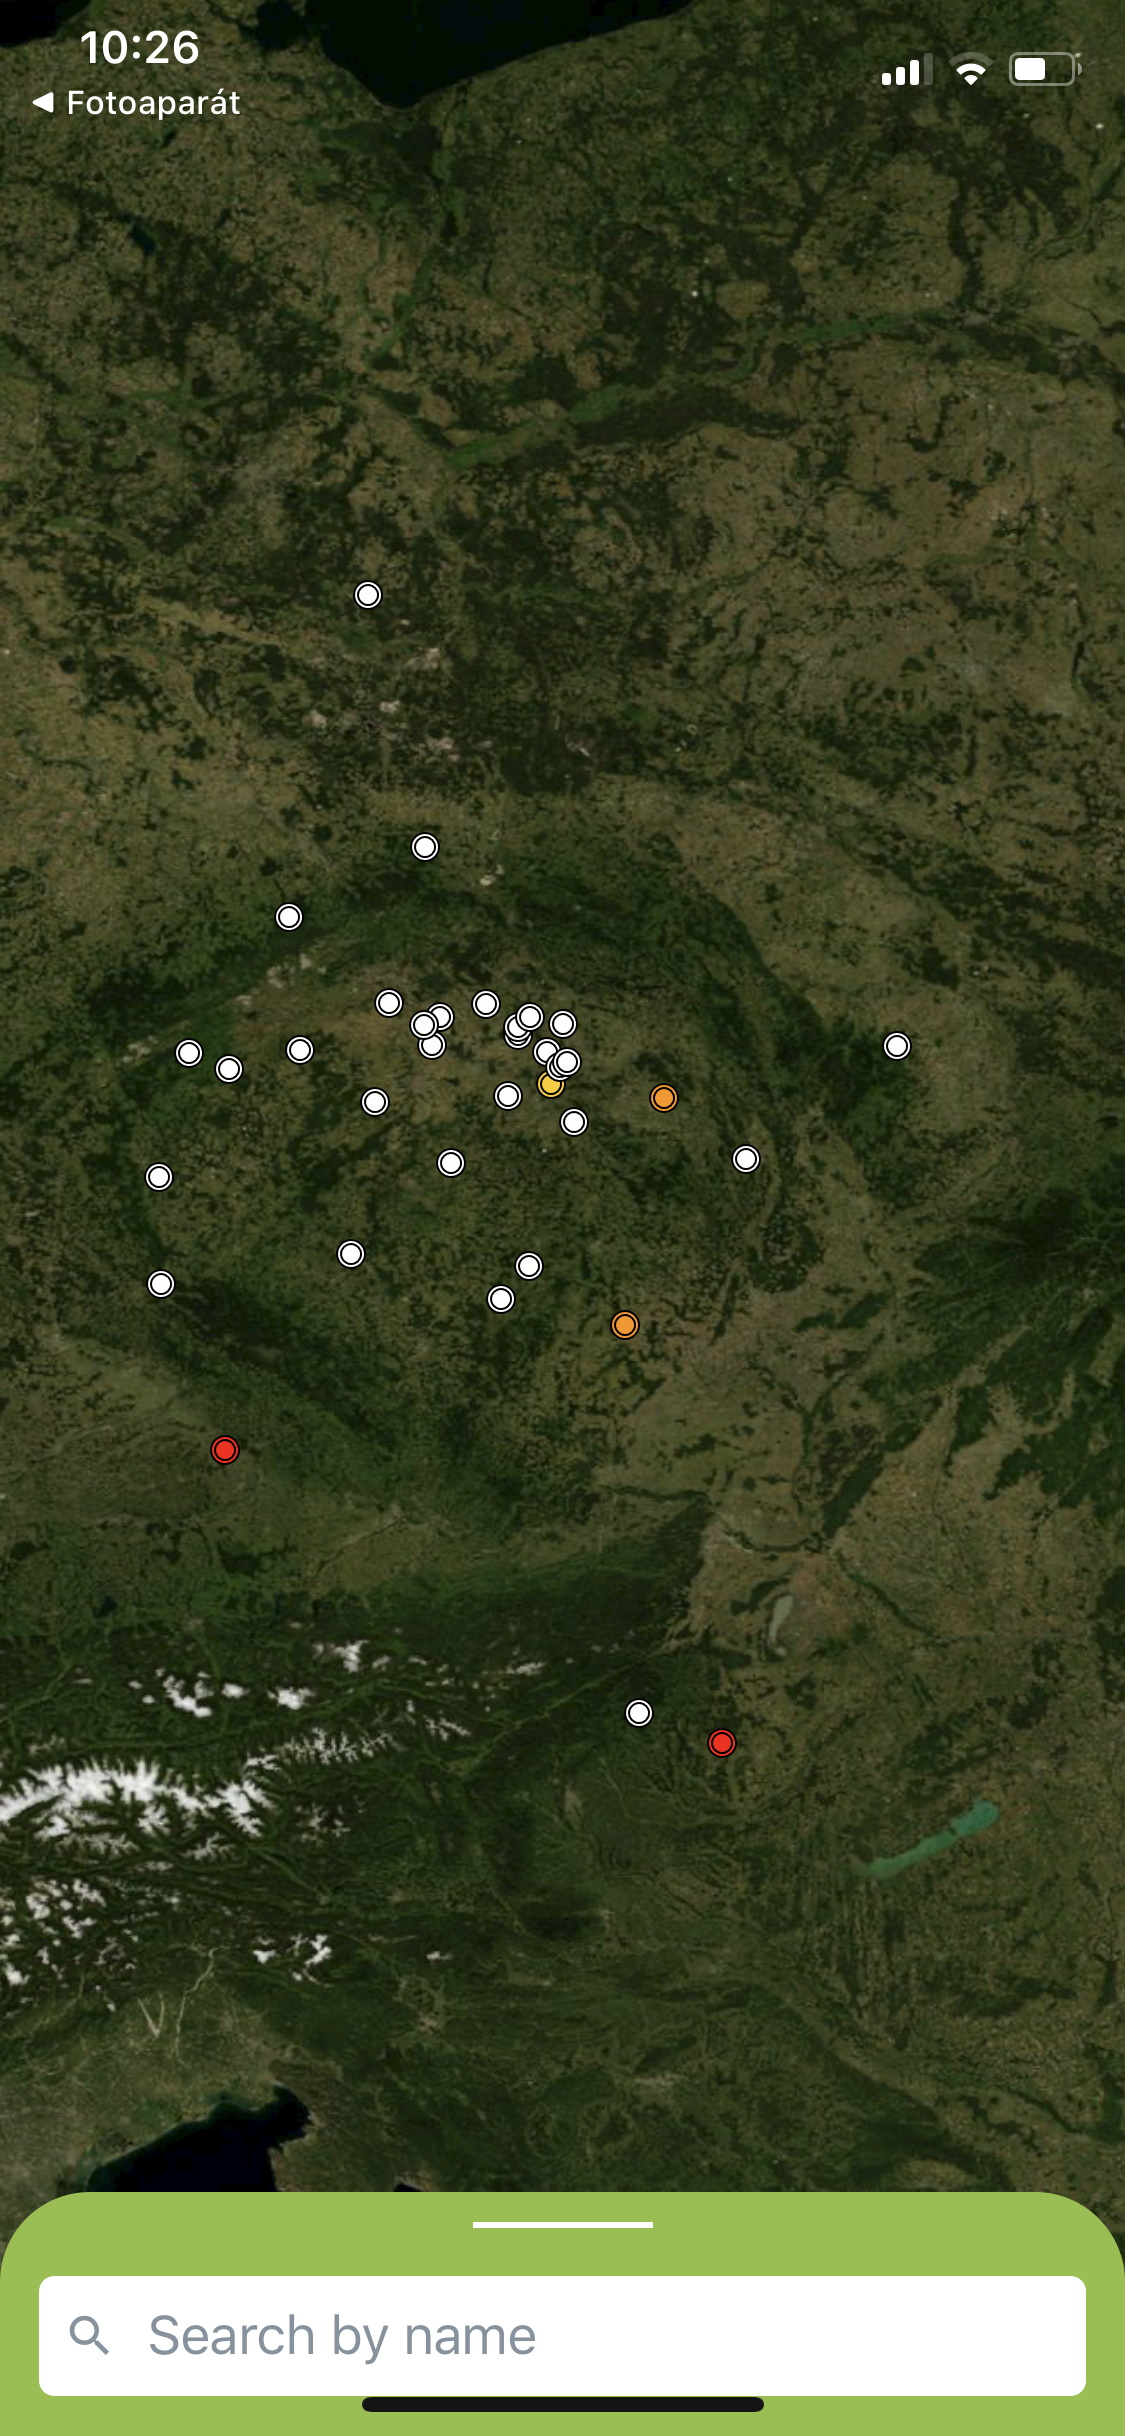
\includegraphics[width=70mm]{img/example_map.jpg}
	\end{center}
	\caption[Výsledek implementace hlavní mapy]{Výsledek implementace hlavní mapy -- zdroj: autor}
\end{figure}

Výsledek implementace mapy je srovnatelný s drátěným modelem představeným v kapitole Návrh.

\section{Implementace subkomponent}

Subkomponenty byly vytvořeny pro splnění mapové koncepce, tedy pro jednotlivé overlay funkce definované v kapitole návrh. Zbylé subkomponenty byly vytvářeny dle potřeby pro zpřehlednění aplikace, tedy ad hoc. Za zvláštní zmínku stojí implementace off-line map, která byla vytvořena čistě pro tuto aplikaci.

\subsection{Implementace off-line map}

Pro implementace off-line map bylo nutno vytvořit dvě komponenty. První komponentou jsou off-line mapy samotné, druhou komponentou způsob, jak vybrat rozsah, který má být stažen.

Off-line schopnost map je umožněna díky následujícím klíčovým možnostem: možnost načítat tzv. tile mapy (mapy uložené ve formátu obrázků s jednoznačným indexem v dimenzích x, y a z) a URI, které využívá Expo i pro ukládání souborů. Pro mapy je tedy jedno, zda načítají jednotlivé mapové čtverečky z disku, či přímo ze vzdáleného mapového serveru.

\begin{lstlisting}[language=JavaScript, caption=Off-line mapy]
import { UrlTile } from 'react-native-maps';
<MapView..>
	<UrlTile urlTemplate="..."/>
</MapView>
\end{lstlisting}

Do urlTemplate se místo vzdáleného zdroje doplní část kódu, která obsahuje parametry pro jednotlivé dimenze mapy ve formátu \emph{\{z\}/\{x\}/\{y\}.png}. Každý mapový čtvereček je následně načítán z disku. Toto chování je vhodné zapnout pouze v případě že uživatel není připojený k síti, či na přímé vyžádání uživatele.

Kvůli nedostatku času nebylo možné vytvořit komfortní uživatelský nástroj pro výběr off-line map, a vznikl proto pouze rudimentární. Z kontextového menu uživatel zapne dialog zadávání bodů, čímž se uloží příznak do aplikace, že uživatel vybírá off-line region. Uživatel je následně instruován, aby klikal do mapy.

\section{Implementace navigátorů}

Pro implementaci navigátorů byla vybrána již zmiňovaná standardní knihovna\linebreak \emph{react-navigation}, pro instalaci je využitý balíčkovací nástroj NPM.

\begin{lstlisting}[language=Bash, caption=Instalace react-navigation]
npm install react-navigation
npm install react-navigation-stack
\end{lstlisting}

Po instalaci je nejprve ve vybrané React komponentě nejprve naimportovat dané knihovny. 

\begin{lstlisting}[language=JavaScript, caption=Import knihoven pro hlavní navigátor]
import { createSwitchNavigator, createAppContainer, NavigationContainerComponent, NavigationActions } from 'react-navigation';
import { createStackNavigator } from 'react-navigation-stack';
\end{lstlisting}

Importováním těchto závislostí půjde vytvořit switch navigátor, hlavní navigační kontejner aplikace a stack navigátor. Následně je nutné naimportovat komponenty obrazovek následujícím způsobem.

\begin{lstlisting}[language=JavaScript, caption=Import obrazovek pro hlavní navigátor]
import Welcome from './src/screens/auth/Welcome'; // naimportuje komponentu obrazovky Welcome
import Login from './src/screens/auth/Login';
import Register from './src/screens/auth/Register';
import MapScreen from './src/screens/in/Map';
\end{lstlisting}

Navigátory lze následně sestavit modulárním způsobem vkládání do sebe, kde listy grafu navigátorů jsou jednotlivé komponenty obrazovek.

\begin{lstlisting}[language=JavaScript, caption=Implementace navigátorů]
const AuthContainer = createStackNavigator({
	Welcome: Welcome,
	Login: Login,
	Register: Register
}, {
	headerMode: 'none'
});

const AppNavigator = createSwitchNavigator({
	AuthLoading: AuthLoading,
	Map: MapScreen,
	AuthContainer: AuthContainer
}, {
	"initialRouteName": "AuthLoading" // nazev vychozi cesty, resp. obrazovkove komponenty
});
\end{lstlisting}

Navigátory se následně obalí aplikačním kontejnerem, ze kterého se vytvoří hlavní komponenta aplikace, tedy její vstupní bod.

\begin{lstlisting}[language=JavaScript, caption=Vytvoření aplikačního kontejneru]
const AppContainer = createAppContainer(
	AppNavigator
);

export default class App extends React.Component
{
	render () {
		return (
				<React.Fragment>
					<AppContainer ref = { setNavigatorRef }/>
					<FlashMessage position="top" />
				</React.Fragment>
		)
	}
}
\end{lstlisting}

V ukázce kódu se vytváří komponenta App, která je vstupním bodem aplikace. V komponentě App se nachází fragment, který je kolekcí různých React komponent a sám nemá v uživatelském rozhraní žádnou funkci. Následně se vytvořený AppContainer využije přímo v komponentě a jeho vykresleným obsahem se stávají různé obrazovky specifikované v předchozích ukázkách kódu. Ačkoliv se nejedná přímo o funkce navigátoru, na stejné úrovni se také nachází komponenta FlashMessage, která zajistí, že se tzv. flash zprávy vygenerované v aplikaci zobrazují napříč všemi obrazovkami z jednoho místa (tedy bez duplikace kódu). Nejedná se tedy o funkci navigátoru, ale pouze o komponentu, kterou je vhodné umístit na nejvyšší úroveň kvůli prevenci duplikaci kódu a jedná se o vhodnou ukázku, co lze na stejnou úroveň jako kontejner navigátorů vložit.

Pro přenavigování lze využít v jakékoliv komponentě umístěné pod AppContainerem (resp. pod jakýmkoliv navigátorem) funkcí uvedenou níže.

\begin{lstlisting}[language=JavaScript, caption=Přenavigování]
this.props.navigation.navigate("Map");
\end{lstlisting}

Všem komponentám je předán odkaz na navigátor a pomocí klíče (názvu) obrazovky se na ni lze přenavigovat kdekoliv uvnitř komponenty, např. při reagování na kliknutí z tlačítka či doběhnutím vnitřní události. Navigace mimo komponentu ale tímto způsobem není možná, proto byl autorem aplikace v App.tsx vytvořena možnost, jak tuto funkci z komponenty získat. V komponentě AppContainer byl specifikován atribut ref. Atribut ref v Reactu slouží k získání instance určité komponenty. Komponenta se předá funkci setNavigatorRef, který do lokální proměnné vloží instanci navigátoru. Aplikace nad touto lokální instancí vytváří funkci navigate, ve které volá událost navigace a je tedy možné z kódu mimo komponenty volat funkce navigace.

\begin{lstlisting}[language=JavaScript, caption=Přenavigování]
let instanceRef: NavigationContainerComponent;

function setNavigatorRef(instance: NavigationContainerComponent) {
	instanceRef = instance;
}

function navigate(routeName, params) {
	instanceRef.dispatch(
		NavigationActions.navigate({
			routeName,
			params,
		})
	);
}
\end{lstlisting}

\section{Implementace push notifikací}

Jednou z mnoha výhod platformy Expo je jednoduchost napojení aplikačních push notifikací. Není potřeba využívat různé poskytovatele pro různé platformy, Expo zajistí doručení na jakékoliv zařízení, které se k notifikacím registruje. Výhodou také je jednoduchost celého systému, kde stačí aby se zařízení pouze oznámilo serveru svým identifikátorem a následně lze notifikace volat za pomocí REST API Expo. Celý proces je velmi jednoduchý na implementaci v mobilní aplikaci i ve zdroji notifikací. Získání notifikací na straně aplikace lze docílit následujícím způsobem.

\begin{lstlisting}[language=JavaScript, caption=Expo notifikace]
import { Notifications } from 'expo';
import * as Permissions from 'expo-permissions';
import Constants from 'expo-constants';


const { status } = await Permissions.askAsync(Permissions.NOTIFICATIONS);

if (finalStatus !== 'granted') {
	return;
}

const token = await Notifications.getExpoPushTokenAsync();
\end{lstlisting}

Pro notifikace je třeba získat svolení uživatele. Pokud svolení dá, Expo vrátí textový token, který se následně dá použít k poslání notifikace na konkrétní zařízení. Pro zjednodušení práce s větším počtem stejných notifikací je možnost vytvářet skupiny příjemců, aplikace ji nevyužívá. Kód pro generování zpráv na straně serveru není součástí této práce a je pouze obsažen ve webovém backendu aplikace Anitra.

% \section{Sestavení pomocí TurtleCLI}

% \section{Publikování na Google Play}